\chapter{磁场}

\section{磁场和磁感应强度}

人们最早发现的天然磁石的主要成份是$Fe_3O_4$ .现在使用的磁体,多是用铁、钴、镍等金属或用某些氧化物制成的.天然磁石和人造磁体都叫做{\bf 永磁体},它们都能吸引铁质物体,我们把这种性质叫做{\bf 磁性(magnetism)}.磁体的各部分磁性强弱不同,磁性最强的区域叫做{\bf 磁极(magnetic ploe)}.能够自由转动的磁体,例如悬吊着的磁针,静止时指南的磁极叫做南极,又叫$S$极;指北的磁极叫做北极,又叫$N$极.
\footnote{引用自人教版高中物理选修3---1.其中$S$极和$N$极这两个字母分别指 south 和north.}

磁体周围存在磁场,磁场对放入磁场中的磁体或电流有力的作用.按当前的理论,磁场的产生是由于微观电流,而电场的产生是因为电荷,所以研究磁场就不能像研究电场一样定义磁场强度,原因是不存在像电荷一样的粒子导致磁场(这样的粒子叫做磁单极子,现实中不存在.),所以在规定磁场的方向和大小上就与电场产生了不同地方.

\subsection{磁感应强度B的方向}

由于不存在磁单极子,同时对于放入磁场中的磁体会受到力的作用,所以我们也像研究电场一样使用磁感应强度来描述磁场力的性质.这里大家注意,之所以使用磁感应强度而不使用磁场强度,因为在历史上对磁的认识有错误,而磁场强度已经由另外一个量使用了,所以这里就按照历史的叫法沿用下来而对磁场力的性质使用磁感应强度来描述.磁感应强度的符号为$B$,它是一个矢量,单位是{\bf 特斯拉}, 符号为$T$.磁体上在两个磁极,我们规定将小磁针放入磁场中,当它平衡时,小磁针北极(N极)所指的方向为磁感应强度$B$ 的方向.

\subsection{磁感应强度B的大小}

当磁体放入磁场时,会受到力的作用.但是由于磁单极子不存在,我们就不能像定义电场强度那样来定义磁感应强度.但是当电流放入磁场时也会受到力的作用,而且对于导线的长度及电流的大小也是可控的,这样我们就可以使用电流来定义磁感应强度的大小.这里需要注意,由于电流的周围也会形成磁场,所以像定义电场时所采用的试探电荷一样,这里使用的电流必然不能太大,导线的长度也不能太长,原因就是不能使来探测的电流干扰原来的磁场.像这样的长度很小,同时电流又不大的通电导线,我们称之为电流元,它的大小为$I\Delta L$ ,其中$I$ 为电流大小,$\Delta L$ 为导线的长度.但是当这个电流元放入磁场时,它受到的力不是一成不变的,当电流元的方向(小导线中电流的流向)与磁感应强度$B$的方向垂直时它受到的力最大,此力记为$F$,我们定义这个最大的力与电流元的比值为磁感应强度,即
\begin{equation}
  B=\frac{F}{I\Delta L}
  \label{eq:magneticB}
\end{equation}

\section{几种常见的磁场}

在磁场中我们定义了磁感应强度$B$来描述磁场力的性质,像描述电场一样我们用一些假想的曲线来描述磁场,这些假想的曲线叫做磁感线(magnetic induction line).使用磁感线来描述磁场,可以使我们获得一些比较直观的认识.这里我们列出磁感线的一些性质:

\begin{enumerate}
  \item 磁感线是闭合曲线,在磁体的外部,磁感线由$N$极指向$S$极,在磁体的内部,磁感线由$S$极指向$N$极,而形成闭合曲线.\footnote{大家注意,电场线是起于正电止于负电,它是不闭合的曲线,电场线和磁感线是不同的.}
  \item 磁感线的疏密表示磁感应强度的大小.
  \item 磁感线切线的方向就是磁感应强度$B$ 的方向.
  \item 任意两条磁感线不相交,因为$B$的方向是唯一的,如果相交,则在交点处的$B$就有两个方向了.
  \item 任意两条感线也不相切.因为磁感线的疏密表示大小,而相切的话,则切点处将会是密不可分的,也就是$B$无穷大的状态,这在物理上也是不允许的.
\end{enumerate}

\subsection{一些常见的磁体的磁感线}

\begin{figure}[H]
  \centering
  \includegraphics{./cichang/图片1.png}
  \qquad
  \includegraphics{./cichang/图片2.png}
  \caption{条形磁铁和蹄形磁铁}
\end{figure}
条形磁铁和蹄形磁铁是最常见的两类磁铁,其中蹄形磁铁两个磁极间的部分可以视为匀强磁场,即可以近似为等间距的平行线.这也是在以后各类计算题中经常出现的情况.


\begin{figure}[H]
  \centering
  \includegraphics{./cichang/图片3.png}
  \caption{无限长直线电流的磁场}
\end{figure}
无限长直线电流的磁场:让右手握住导线,让伸直的拇指所指的方向与电流方向一致,弯曲的四指所指的方向就是\CJKunderwave{磁感线环绕的方向}. 这个规律也叫做右手定则.这里我们给大家指明一点,在以后我们还要计算安培力和洛仑兹力,它们的方向要用左手定则来判定,这时就有同学混淆了左手和右手的适用范围,我这样给大家解释:\CJKunderwave{在中国通常都是男左女右,而男生比较有力气,所以判定力的时候就是左手定则,其它的情况就是右手了.}这种磁场的特点是:以导线上各点为圆心的同心圆,圆所在的平面与导线{\bf 垂直},越向外{\bf 越疏}.

\begin{figure}[H]
  \centering
  \includegraphics{./cichang/图片4.png}
  \caption{环形电流的磁场}
\end{figure}
环形电流的磁场:让右手弯曲的四指与\CJKunderwave{环形电流}的方向一致,伸直的拇指所指的方向就是\CJKunderwave{环形导线轴线}上磁感线的方向.其特点:内部比外部强,磁感线越向外越疏.

\begin{figure}[H]
  \centering
  \includegraphics{./cichang/图片5.png}
  \caption{通电螺线管的磁场}
\end{figure}
通电螺线管的磁场:用右手握住螺线管,让弯曲的四指指向\CJKunderwave{电流}的方向,那么\CJKunderwave{大拇指}所指的方向就是螺线管中心轴线上磁感线的方向.其特点为:内部为\CJKunderwave{匀强磁场},且内部比外部强.内部磁感线方向由\CJKunderwave{S极}指向 \CJKunderwave{N极},外部由\CJKunderwave{N极}指向\CJKunderwave{S极}.

\subsection{安培分子电流假说}

安培分子电流假说认为:在原子,分子等物质微粒的内部,存在着一种环形电流------分子电流.分子电流相当于一个小磁针,它使每个物质微粒都成为微小的磁体,它的两侧相当于两个磁极.

\begin{figure}[H]
  \centering
  \includegraphics{./cichang/图片6.png}
  \caption{安培分子电流假说}
  \label{fig:anpeiI}
\end{figure}

如图\ref{fig:anpeiI}所示,当铁棒中分子电流的取向\CJKunderwave{大致相同}时,铁棒对外显磁性(如甲所示);当铁棒中分子电流的取向变得\CJKunderwave{杂乱无章}时,铁棒对外不显磁性(如图乙所示).安培分子电流假说说明\CJKunderwave{一切磁现象都是由电荷的运动产生的.}
\section{安培力}

当一段导线放入磁场中时会受到力,这个力叫做安培力.最简单的一种情况,是长直导线放入匀强磁场中,且满足导线与磁感应强度的方向相互垂直.如图\ref{fig:anpeiforce}所示,空间中充满垂直于纸面向里的匀强磁场,磁感应强度大小为$B$,在磁场中存在一根无限长直导线(无限长是相对于磁场来说的),导线的长度为$L$,导线中通有恒定电流,电流大小为$I$.

\begin{figure}[H]
  \centering
  \begin{tikzpicture}
    \foreach \x in {-1.4,-1,-0.6,-0.2,0.2,0.6,1,1.4} 
    \foreach \y in {-1.4,-1,-0.6,-0.2,0.2,0.6,1,1.4} 
    \draw (\x,\y) node {\small $\times$};
    \draw (-0.1,-1.2)--(-0.1,1.2);
    \draw (0.1,-1.2)--(0.1,1.2);
    \draw [->,>=stealth] (0,-0.5)--(0,0.5);
    \foreach \y in {-1.2,-0.9,-0.6,-0.3,0,0.3,0.6,0.9,1.2}
    \draw (-0.1,\y)--(0.1,\y);
    \foreach \y in {-1.2,-0.6,0,0.6,1.2}
    \draw[pattern=north west lines] (-0.1,\y) rectangle ++(0.2,0.3);
    \foreach \y in {-1.05,-0.75,-0.45,-0.15,0.15,0.45,0.75,1.05,1.35}
    \draw [->,>=stealth](0,\y)--++(-1,0) node [anchor=east] {\small $f$};
    \draw (0,-1.8) node [anchor=north] {\small 甲};
  \end{tikzpicture}
  \qquad
  \begin{tikzpicture}
    \foreach \x in {-1.4,-1,-0.6,-0.2,0.2,0.6,1,1.4} 
    \foreach \y in {-1.4,-1,-0.6,-0.2,0.2,0.6,1,1.4} 
    \draw (\x,\y) node {\small $\times$};
    \draw (-0.1,-1.2)--(-0.1,1.2);
    \draw (0.1,-1.2)--(0.1,1.2);
    \draw [->,>=stealth] (0,-0.5)--(0,0.5);
    \draw[->,>=stealth] (0,0)--++(-1.5,0) node [anchor=east]{\small $F$};
    \draw (0,-1.8) node [anchor=north] {\small 乙};
  \end{tikzpicture}
  \caption{安培力}
  \label{fig:anpeiforce}
\end{figure}

在图甲中, 我们可以将无限长直导线视为若干段相同的电流元,由于每一段电流元所处的环境是完全相同的,所以它们的受力情况也完全相同,即大小和方向都相同,按照磁感应强度$B$的定义,我们可以得到每一电流元的所力大小为$BI\Delta L$.然后我们将这无数个小电流元所受力叠加起来,则得到整个导线受到的力,由于匀强磁场和恒定电流,则$B$和$I$均是常量,则各力的方向又相同,所以叠加的结果就是各电流元的长度相加,而整体受力的方向与每一个小电流元受力方向相同,使用左手定则来判定即可.所心可得整个导线受到的力------安培力为
\begin{equation}
  F=BIL
  \label{eq:anpeiforce}
\end{equation}

\section{运动电荷在磁场中受到的力}

带电粒子在磁场中运动时相当于形成了电流,而电流在磁场中会受到力的作用,因此单个粒子在磁场中运动就会受到力的作用. 这一节我们的目标就是求出这个力的表达形式.考虑一个由全部相同的带电粒子所构成的电流元放入磁场中,由于是电流元所以其体积很小,其所处的磁场就可以视为匀强磁场,而电流元的电流恒定,由于所有带电粒子相同,所以在微观看来,每个带电粒子所处的环境是相同的,则每一个电荷所受到的力的大小和方向应当是一致的.因此,\CJKunderwave{电流元所受到力的方向就和单个电荷受力方向一致},这可以由左手定则来判定.其大小应当等于\CJKunderwave{电流元受力除以电流元中所含电荷的数目.}设电流元中电荷总数为$N$,电流元的长度为$\Delta L$,单位体积内电荷数目为$n$,每个电荷的带电量为$q$, 在所考虑的点上磁感应强度为$B$,则
\begin{gather}
 N=nS\Delta L 
 \label{eq:lorentz0}
 \intertext{由电流的微观定义式可得}
 I=nqvS
 \label{eq:lorentz1}
 \intertext{由式\eqref{eq:lorentz0}和式\eqref{eq:lorentz1}联立可以将电流元内的总电荷数用电流表达出来,为}
 N=\frac{I\Delta L}{qv}
 \label{eq:lorentz2}
 \intertext{电流元受力,由磁感应强度的定义可得为}
 F=BI\Delta L
 \label{eq:lorentz3}
 \intertext{由前述分析可得,每一个带电粒子所受力的大小为}
 f=\frac{F}{N}=qvB
 \intertext{所以我们就求出了一个带电粒子在磁场中所受到的力,这个力叫做洛仑兹力,重书如下}
 f=qvB
 \label{eq:lorentz4}
\end{gather}
{\bf 注意} 当我们判断洛仑兹力的方向时,使用左手定则,应当使磁感线由手掌穿入,手背穿出,四指指向\CJKunderwave{电荷所\CJKunderdot{形成电流}的方向},则拇指所指的方向就是洛仑兹力的方向.

我们注意,在上述讨论中我们使用的磁感应强度的定义来求出的电流元所受的力,仔细考虑这个问题,多少有些不严格,因为我们不能保证电流元放磁场时就一定与磁场垂直,此时我们再来讨论一下电流元与磁场不垂直的情况,如图\ref{fig:lorentz0}所示

\begin{figure}[H]
  \centering
  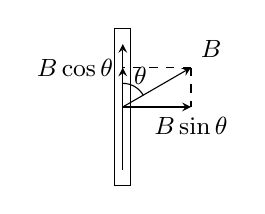
\begin{tikzpicture}
    \draw (-0.1,-1) rectangle (0.1,1);
    \draw[->,>=stealth] (0,-0.8)--(0,0.8);
    \draw [->,>=stealth] (0,0)--++(30:1) node [anchor=south west] {\small $B$};
    \draw [->,>=stealth] (0,0)--(0.866,0);
    \draw [->,>=stealth] (0,0)--(0,0.5);
    \draw[dashed](0,0)++(30:1)--++(0,-0.5) node [anchor=north] {\small $B\sin\theta$};
    \draw[dashed](0,0)++(30:1)--++(-0.866,0) node [anchor=east] {\small $B\cos\theta$};
    \draw (30:0.3) arc (30:90:0.3);
    \draw (60:0.45) node {\small $\theta$};
  \end{tikzpicture}
  \caption{电流元与磁场不垂直的情况}
  \label{fig:lorentz0}
\end{figure}

我们可以将磁感应强度$B$ 分解为与电流垂直的分量$B\sin\theta$ 和与电流平行的分量 $B\cos\theta$ ,但是平行分量对电流元无力的作用,只有垂直分量有力的作用,则此时电流元所受力的大小为
\begin{gather}
 F=I\Delta L\cdot B\sin\theta 
 \intertext{所以每个带电粒子在此时所受力的大小为}
 f=\frac{F}{N}
 \intertext{关于$N$的计算同前述一致,则洛仑兹力大小为}
 f=qvB\sin\theta 
 \label{eq:lorentz5}
\end{gather}
显然式\eqref{eq:lorentz5}是比\eqref{eq:lorentz4}更加普遍的表达式,如果令$\theta=\frac{\pi}{2}$,则就由式\eqref{eq:lorentz5}得到了式\eqref{eq:lorentz4}.

\section{带电粒子在匀强磁场中的运动}

上一节我们求出了洛仑兹力的表达式,确定了它的受力方向.如果带正电的粒子处于匀强磁场中,且速度方向与磁场垂直.则如图\ref{fig:lorentz1}所示

\begin{figure}[H]
  \centering
  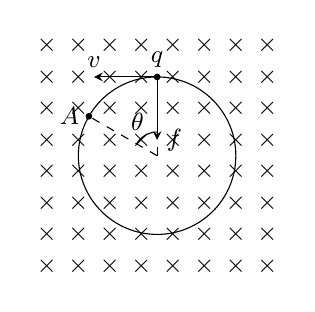
\begin{tikzpicture}
    \foreach \x in {-1.4,-1,-0.6,-0.2,0.2,0.6,1,1.4} 
    \foreach \y in {-1.4,-1,-0.6,-0.2,0.2,0.6,1,1.4} 
    \draw (\x,\y) node {\small $\times$};
    \draw (0,0) circle [radius=1];
    \filldraw (0,1) circle [radius=1pt] node [anchor=south]{\small $q$};
    \draw[->,>=stealth] (0,1)--++(-0.8,0) node [anchor=south] {\small $v$};
    \draw[->,>=stealth] (0,1)--++(0,-0.8) node[anchor=west] {\small $f$};
    \draw[dashed](0,0)--++(90:1);
    \draw[dashed](0,0)--++(150:1);
    \filldraw (150:1) circle [radius=1pt] node [anchor=east] {\small $A$};
    \draw(90:0.3) arc (90:150:0.3);
    \draw(120:0.5) node {\small $\theta$};
  \end{tikzpicture}
  \caption{带电粒子在磁场中运动}
  \label{fig:lorentz1}
\end{figure}

由于洛仑兹力与速度每时每刻都垂直,所以我们可以得到结论:\CJKunderwave{洛仑兹力不做功}.在图\ref{fig:lorentz1}中速度与磁感应强度垂直,同时由左手定则可得,力也同时与速度和磁感应强度垂直,由于洛仑兹力不做功,显然带电粒子做\CJKunderwave{匀速直线运动}.我们的任务是计算出描述圆周运动的一些物理量.在圆周运动中起核心作用的就是角速度,所以我们先求解角速度,由牛顿第二定律得
\begin{gather}
 mv\omega=qvB 
 \intertext{解得}
 \omega=\frac{qB}{m}
\end{gather}
如图\ref{fig:lorentz1}中,带电粒子从开始的$q$ 位置运动到$A$位置 ,设其所用时间为$t$,则由圆周运动可得
\begin{gather}
  t=\frac{\theta}{\omega}\notag
  \intertext{代入角速度表达式可得}
  t=\frac{\theta m}{qB}
\end{gather}
 我们注意到,如果记转一周的时间为$T$,则它就是带电粒子做匀速圆周运动的周期,则
 \begin{gather}
   T=\frac{2\pi m}{qB}
 \end{gather}
 如果线速度$v$的大小已知,则由线速度与角速度的关系可得
\begin{gather}
  r=\frac{v}{\omega}\notag
  \intertext{代入角速度表达式得}
  r=\frac{mv}{qB}
\end{gather}

\subsubsection{质谱仪}

在自然界中有许多化学元素存在同位素,同位素的质子数相同,所以化学反应相同,但是它们的中子数不同,所以它们的物理反应是不同的.利用带电粒子在电磁场中做匀速圆周运动,可以区分同位素.如图\ref{fig:zhipuyi0}所示

\begin{figure}[H]
  \centering
  \includegraphics{./cichang/图片7.png}
  \caption{质谱仪}
  \label{fig:zhipuyi0}
\end{figure}

一个质量为$m$、电荷量为$q$的粒子,从容器$A$下方的小孔$S_1$飘入电势差为$U$ 的加速电场,其初速度几乎为$0$ ,然后经过$S_3$ 沿着与磁场垂直的方向进入磁感应为$B$ 的匀强磁场中,最后打到照相底片$D$上(图 \ref{fig:zhipuyi0}).求粒子在磁场中运动的轨道半径.

上面这道题是选自课本选修3---1 第100页 上的例题.为了求半径,我们根据带电粒子在磁场中运动时半径的表达式可知,首先我们需要求出速度$v$,根据动能定理可得
\begin{gather}
  qU=\frac{1}{2}mv^2-0
  \intertext{解得}
  v=\sqrt{\frac{2qU}{m}}
\end{gather}
由半径与线速度的关系可得
\begin{gather}
  r=\frac{mv}{qB}
  \intertext{将线速度代入上式得}
  r=\frac{m}{qB}\cdot\sqrt{\frac{2qU}{m}}
  \intertext{简单整理得}
  r=\frac{1}{B}\sqrt{\frac{2mU}{q}}
\end{gather}
由半径的表达式可得,只要带电粒子的比荷$\frac{q}{m}$ 相同,则粒子的轨迹半径就是相同的.比荷大的粒子,半径相应的小,从左侧底片上刻好刻度,则就能根据刻度来识别不同的同位素.

\subsubsection{回旋加速器}

在研究带电粒子的性质时,往往我们需要使用粒子相互撞击来了解一些粒子的信息.这就涉及到加速带电粒子的问题.通常需要粒子加速到很大的能量才能使粒子对撞而产生新的粒子等,根据动能定理,即
\begin{gather}
  qU=\frac{1}{2}mv^2
\end{gather}
我们可以通过电场加速粒子,而使其获得相应的动能.但是这里有一个问题就是,通常我们日常使用的电压是不会达到很高的,所以一次性加速粒子不能使其获得足够的能量.于是需要我们多次加速同一粒子.理论上我们可以使粒子通过多组平行板加速器,但是这在理论上可行,如果这样做的话,我们需要的设备过于庞大.但是我们注意到带电粒子在磁场中运动时其角速度($\omega=\frac{qB}{m}$)与线速度是无关的,进而粒子做匀速圆周运动的周期无论线速度多大都不发生变化.根据这一特殊的原理,美国著名物理学家 欧内斯$\cdot$劳伦斯(Ernest Orlando Lawrence)于1932年设计和制造了第一台高能粒子回旋加速器.如图\ref{fig:huixuanjiasu0}所示,是回旋加速器的原理图.

\begin{figure}[H]
  \centering
  \includegraphics{./cichang/图片8.png}
  \caption{回旋加速器}
  \label{fig:huixuanjiasu0}
\end{figure}

回旋加速器由两个正对$D$ 型盒构成,在与两个$D$ 型盒正对的缝垂直的同时与$D$ 型盒的大表面平行的电场,由于静电屏蔽作用,则盒内部电场为零,但是接缝处电场不为零,并且两个$D$型盒是等势体,则接缝处的电势差在不同位置时都相同.在垂直于$D$ 型盒的方向,我们加上匀强磁场,金属盒不能屏蔽磁场,所以$D$型盒内部是存在匀强磁场的.所以带电粒子在$D$型盒内做匀速圆周运动,同时每半个周期粒子就穿过接缝,这里必须使电场与粒子的运动同步的改变正负极,这样粒子每次通过接缝就会加速一次.连续工作下去,带电粒子就能在$D$型盒内完成多次加速.最终的速度大小,取决于$D$型盒的半径,即
\begin{gather}
  v_m=R\frac{qB}{m} 
\end{gather}

但是大家注意,并不是此半径越大最终获得的速度越大.因为,当粒子加速到一定的程度后,它的速度若与光速可以比拟(即达到相同数量级),则按照相对论
\footnote{相对论是现今正确的力学理论,我们现在所学的力学实际上是速度远远小于光速的相对论近似,我们把现在大家学习的理论称为经典力学.我们不能说经典力学是错的,因为即便是用严格的相对论来处理问题,我们的公式最终也将近似到经典力学上来,而且作这个近似时,精确度还是相当相当高的.但是在物体高速运动时,经典力学就不适用了,而必须用相对论来解决.}
的理论粒子将会向外辐射电磁波,粒子将不会继续加速.所以现实中,回旋加速器确实实现了在小空间内加速粒子的目的.但是,一旦达到一定的速度它将不能再加速粒子,但是在回旋加速器后再追加若干组直线加速器,则粒子就可以继续加速.所以实现超高能的粒子,还需要直线加速器的.

为了清析的完成计算,我们画出俯视图如图\ref{fig:huixuanjiasu1}所示.我们知道,粒子每经过一次电场,则动能增加$qU$,带电粒子最初的速度接近为零,所以假设加速了$n$次,则最后的动能为$nqU$,所以可以求出加速$n$ 次的速度为
\begin{gather}
  nqU=\frac{1}{2}mv_n^2\notag
  \intertext{解得}
  v_n=\sqrt{\frac{2qU}{m}}\cdot \sqrt{n}
  \intertext{所以加速$n$次后的半径为}
  r_n=\frac{mv_n}{qB}=\frac{1}{B}\sqrt{2mU}{q}\cdot\sqrt{n}
  \intertext{所以各半径之比为}
  r_1:r_2:r_3:\cdots:r_n=\sqrt{1}:\sqrt{2}:\sqrt{3}:\cdots:\sqrt{n}
  \intertext{加速两次造成的半径变化为}
  \Delta r=r_1(\sqrt{n}-\sqrt{n-1})
\end{gather}
由此可得速度越大的时候半径差距越小.极限情况是最后的半径相同.这带来的好处是:轨道越来越密集,则可以将$D$形盒设计的更小一些.同时,最终的半径近似可以认为相同,而圆心近似在$D$形盒的中心.图\ref{fig:huixuanjiasu1}就是根据这个根号比严格画出来的图,我们设$D$型盒的半径为$R$,所以可以由此半径求出最大的速度$v_m$.

\begin{figure}[H]
  \centering
  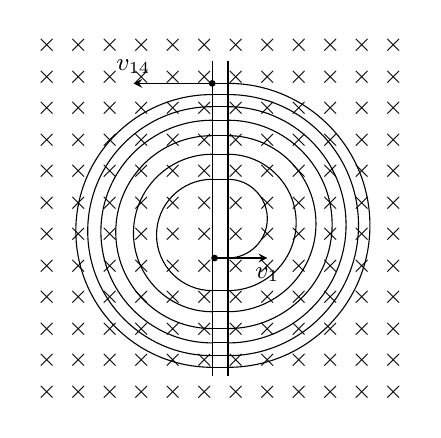
\begin{tikzpicture}
    \foreach \x in {-0.1,0.1} 
    \draw (\x,-2)--(\x,2);
    \filldraw (-0.07,-0.5) circle [radius=1pt];
    \draw (-0.07,-0.5)--(0.1,-0.5);
    \draw [->,>=stealth] (0.1,-0.5)--++(0.5,0) node [anchor=north]{\small $v_1$};
    \draw (0.1,-0.5) arc (-90:90:0.5);
    \draw (0.1,0.5)--(-0.1,0.5);
    \draw (-0.1,0.5) arc (90:270:0.707);
    \draw (-0.1,-0.914)--(0.1,-0.914);
    \draw (0.1,-0.914) arc (-90:90:0.866);
    \draw (0.1,0.818)--(-0.1,0.818);
    \draw (-0.1,0.818) arc (90:270:1);
    \draw (-0.1,-1.182)--(0.1,-1.182);
    \draw(0.1,-1.182) arc (-90:90:1.118);
    \draw (0.1,1.054)--(-0.1,1.054);
    \draw (-0.1,1.054) arc (90:270:1.225);
    \draw (-0.1,-1.396)--(0.1,-1.396);
    \draw (0.1,-1.396) arc (-90:90:1.323);
    \draw (0.1,1.25)--(-0.1,1.25);
    \draw (-0.1,1.25) arc (90:270:1.414);
    \draw (-0.1,-1.578)--(0.1,-1.578);
    \draw (0.1,-1.578) arc (-90:90:1.5);
    \draw (0.1,1.422)--(-0.1,1.422);
    \draw (-0.1,1.422) arc (90:270:1.581);
    \draw (-0.1,-1.74)--(0.1,-1.74);
    \draw (0.1,-1.74) arc (-90:90:1.658);
    \draw (0.1,1.576)--(-0.1,1.576);
    \draw (-0.1,1.576) arc (90:270:1.732);
    \draw (-0.1,-1.888)--(0.1,-1.888);
    \draw (0.1,-1.888) arc (-90:90:1.803);
    \draw (0.1,1.718)--(-0.1,1.718);
    \filldraw (-0.1,1.718) circle [radius=1pt];
    \draw[->,>=stealth] (-0.1,1.718)--++(-1,0) node [anchor=south]{\small $v_{14}$};
    \foreach \x in {-2.2,-1.8,-1.4,-1,-0.6,-0.2,0.2,0.6,1,1.4,1.8,2.2}
    \foreach \y in {-2.2,-1.8,-1.4,-1,-0.6,-0.2,0.2,0.6,1,1.4,1.8,2.2}
    \draw (\x,\y) node {\small $\times$};
  \end{tikzpicture}
  \caption{回旋加速器俯视}
  \label{fig:huixuanjiasu1}
\end{figure}

下面我们来计算,粒子在回旋加速器中速度从$0$ 加速到最后所需要的时间.这个时间我们可以分两部分讨论,其一,粒子在磁场中的时间.其二,粒子在电场中的加速时间.在一般的讨论中由于接缝非常小,且粒子速度越来越大,但是在磁场中做匀速圆周运动的角速度是不变的,所以粒子加速的时间要远小于在磁场中匀速圆周运动的总时间.所以在近似度不是很高的计算中直接认为在磁场中运动的时间就是这个粒子在回旋加速器中的时间.此处,我们将严格来导出这两个时间.由最大速度$v_m$ ,我们可以求出最终的动能
\begin{gather}
  E_m=\frac{1}{2}mv_m^2=\frac{q^2B^2R^2}{2m}
  \intertext{粒子每次加速可以获得动能$qU$,所以总的加速次数$N$ 为}
  N=\frac{E_m}{qU}=\frac{qB^2R^2}{2mU}
  \intertext{由图\ref{fig:huixuanjiasu1}加速一次需要通过一次接缝和完成半个圆周运动,由于是匀速圆周运动,所以加速一次在磁场中用时半个周期$\frac{T}{2}$,我们先写出这个时间$t_1$,则}
  t_1=N\frac{T}{2}=\frac{qTB^2R^2}{4mU}
  \intertext{对于加速部分,由于我们所加电压大小保持不变,所以粒子在电场中做匀加速运动,而在磁场中仅起到一个转向 $180^\circ$ 的作用,所以整体上它和将粒子从 $0$ 直线以相同的加速度加速到 $v_m$ 所需时间是一致的.设接缝的宽度为 $d$,于是我们可以这样等效的求出这个时间$t_2$ }
  t_2=\frac{v_m}{a}=\frac{qBR}{m}\cdot \frac{md}{qU}=\frac{BRd}{U}
  \intertext{则总时间为这两个时间之和.即}
  t=t_1+t_2=\frac{qTB^2R^2}{4mU}+\frac{BRd}{U}
\end{gather}

\subsubsection{速度选择器}

由电场和磁场的配合,我们可以选择粒子的速度,这个设备叫做速度选择器.如图\ref{fig:suduxuanze0}所示,速度选择器由相互垂直的电场和磁场构成,其中磁场垂直于纸面向里,电场由上向下.对于图中所示一个带正电的粒子所受电场力向下,受洛仑兹力向上,如果二个力平衡,则粒子做匀速直线运动,最终通过右侧的出口$O$.如果电场力和洛仑兹力不等,则粒子将会发生偏转,而无法通过最右侧$O$.所以我们就实现的速度选择的目的.下面我们计算一下这个选择的速度,如下
\begin{gather}
 qvB-qE=0
 \intertext{解得}
 v=\frac{E}{B}
\end{gather}
大家注意,速度选择器与粒子的电性是无关的,因为若为负电,则电场力向上,洛仑兹力向下.由于保证平衡,则粒子必须是从左端射入,否则无法达到平衡,也就无法实现速度选择.

\begin{figure}[H]
  \centering
  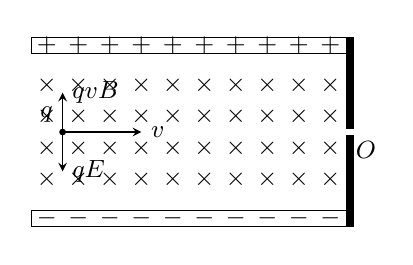
\begin{tikzpicture}
    \draw (-2,-1.2) rectangle (2,-1); 
    \draw (-2,1.2) rectangle (2,1); 
    \filldraw (2,-1.2) rectangle (2.1,-0.05);
    \filldraw (2,1.2) rectangle (2.1,0.05);
    \foreach \x in {-1.8,-1.4,-1,-0.6,-0.2,0.2,0.6,1,1.4,1.8}
    \foreach \y in {-0.6,-0.2,0.2,0.6}
    \draw (\x,\y) node {\small $\times$};
    \foreach \x in {-1.8,-1.4,-1,-0.6,-0.2,0.2,0.6,1,1.4,1.8}
    \draw (\x,-1.1) node {\small $-$};
    \foreach \x in {-1.8,-1.4,-1,-0.6,-0.2,0.2,0.6,1,1.4,1.8}
    \draw (\x,1.1) node {\small $+$};
    \filldraw (-1.6,0) circle [radius=1pt] node [anchor=south east]{\small $q$};
    \draw[->,>=stealth] (-1.6,0)--++(1,0) node [anchor=west]{\small $v$};
    \draw[->,>=stealth] (-1.6,0)--++(0,0.5) node [anchor=west]{\small $qvB$};
    \draw[->,>=stealth] (-1.6,0)--++(0,-0.5) node [anchor=west]{\small $qE$};
    \draw (2,0) node [anchor=north west] {\small $O$};
  \end{tikzpicture}
  \caption{速度选择器}
  \label{fig:suduxuanze0}
\end{figure}

\subsubsection{霍尔元件}

利用带电粒子在磁场中的运动,我们还可以制成探测磁感应强度的仪器---霍尔元件.如图\ref{fig:huoer0}所示,在与恒定电流垂直的方向加以匀强电场$B$,与电流和磁感应强度$B$所在平面平行的两个表面记为$A$和$A'$,两个表面间距离为$h$, 沿磁场方向宽为$d$.

\begin{figure}[H]
  \centering
  \includegraphics{./cichang/图片9.png}
  \caption{霍尔元件}
  \label{fig:huoer0}
\end{figure}

当所加磁场为$B$时,导体中的电荷将会受到洛仑兹力的作用.而向两个表面$A$ 和 $A'$ 偏转,进而形成与磁场和电流都垂直的电场.这就像速度选择器一样,所以当达到平衡时电荷将不再偏转,则$AA'$ 间的电势差将会磁感应强度$B$ 建立一一对应的关系.维持电流$I$不变,则测量$U_{AA'}$ 就能得到此时的磁感应强度$B$.电流的微观定义式为
\begin{gather}
  I=nqvS=nqvdh
  \intertext{解得电荷定向运动的速度$v$为}
  v=\frac{I}{nqdh}
  \intertext{由$AA'$方向受力平衡,可得}
  qvB-qE=0
  \intertext{解得电场强度$E$为}
  E=\frac{IB}{nqdh}
  \intertext{由匀强电场与电势差的关系可得横向电压$U_H$为}
  U_H=Eh=\frac{IB}{nqd}
  \intertext{记$k=\frac{1}{nq}$称为霍尔系数,则}
  U_H=k\frac{IB}{d}
\end{gather}
大家注意,对于不同的粒子,其所形成的电流都是图中所示方向,其不发生变化,所以参与导电的粒子所受洛仑兹力的方向也不发生变化,因此粒子的偏转方向也不发生变化.如正电荷定向移动,则其向$A$侧偏转,导到$U_{AA'}>0$,如负电荷,则也向$A$侧偏转,导致$U_{AA'}<0$,所以由横向电压与零的关系,我们就可以判断参与导电的电荷种类.
\subsubsection{磁流体发电机}

利用带电粒子在磁场中的运动时发生偏转还可以制成发电机---磁液体发电机.如图\ref{fig:ciliutifadian0}所示就是磁流体发电机的原理图.等离子体
\footnote{等离子体:物质是电中性的,当在处于高温时,分子会发生正负电荷的分离,所形成的物质整体电中性,但是由大量的正负离子构成,这种物质就叫做等离子体.}
从左侧射入,正离子所受洛仑兹力方向向上,负离子受洛仑兹力方向向下,因此上极板带正电,下极板带负电,所认在磁流体发电机中上下极板间会形成由上极板指向下极板的电场,因后来的正离子受电场力向下,受洛仑兹力方向向上,则在一段时间后必然会达到平衡.对于负离子,同理也可以达到平衡.当平衡时,离子不再发生偏转,而上下极板会维持一定的电势差,利用这个电势差就可以对外做功.故称磁流体发电机.

\begin{figure}[H]
  \centering
  \includegraphics{./cichang/图片10.png}
  \caption{磁液体发电机}
  \label{fig:ciliutifadian0}
\end{figure}

当等离子体的射入速度恒定时,记为$v_0$, 两板间距离为$d$,所加匀强磁场为$B$,一个离子所带电为$q$,由当平衡时
\begin{gather}
  q\frac{U}{d}=qv_0B
  \intertext{解得}
  U=v_0Bd
\end{gather}

\subsubsection{电磁流量计}

利用带电粒子在磁场中的运动,我们还可以在不破坏管道的情况下进行流量的测定,这个仪器叫做电磁流量计.如图\ref{fig:dianciliuliangji0}所示,为电磁流量计的原理图.

\begin{figure}[H]
  \centering
  \includegraphics{./cichang/图片11.png}
  \caption{电磁流量计}
  \label{fig:dianciliuliangji0}
\end{figure}

我们先来介绍流量的概念.当液体流过一段管道时,我们可以用单位时间内流过横截面的体积来表示液体流动的快慢,这个物理量就是流量.设液体的速度为$v$,横截面积为$S$,流量为$Q$,则
\begin{gather}
  Q=vS
\end{gather}
如图\ref{fig:dianciliuliangji0}所示,管道的半径为$D$,同磁液体发电机一样,我们测得$ab$ 间的电压为$U$,高磁感应强度为$B$, 则
\begin{gather}
  E=\frac{U}{D}\notag\\
  v=\frac{E}{B}\notag\\
  v=\frac{U}{BD}\notag\\
  Q=vS=\frac{U}{BD}\frac{\pi D^2}{4}\notag
  \intertext{解得}
  Q=\frac{\pi DU}{4B}
\end{gather}
所以只要是测得了直径两端的电压$U$,我们就可以根据上述公式得到流量.电磁流量计可以使用的前提是流体内有带电离子,其优点是不用破坏管道的密闭性,比如在核电站中测量重水的流量,由于负责冷却反应堆的水是有辐射的,所以利用电磁流量计来测量流量会更加安全.

\subsubsection{功率仪}

此模型源自于2014年江苏高考题.如图\ref{fig:gonglvyi}所示,导电物质为电子的的霍尔元件位于两串联线圈之间,线圈中电流为$I$,线圈间产生匀强磁场,磁感应强度大小$B$ 与电流$I$ 成正比,方向垂直于霍尔元件的两个侧面,此时霍尔元件的电流为$I_H$, 与其前后表面相边的电压表测出的霍尔电压$U_H$ 满足:$U_H=k\frac{I_HB}{d}$,式中$k$ 为霍尔系数,$d$为霍尔元件两侧面间的距离.电阻$R$ 远大于$R_L$,霍尔元件的电阻可以忽略,则\CJKunderwave{电压表的示数与\mbox{$R_L$}消耗的电功率成正比}.

\begin{figure}[H]
  \centering
  \includegraphics{./cichang/图片13.png}
  \caption{功率仪}
  \label{fig:gonglvyi}
\end{figure}

由于磁感应强度$B$与电流$I$成正比,而电阻$R$和$R_L$ 又是并联,则有
\begin{gather}
  I_H R=(I-I_H)R_L
  \intertext{解得}
  \frac{I_H}{I}=\frac{R_L}{R+R_L}
  \intertext{上式表明$I_H$ 和 $I$ 成正比,同时$I$与$B$成正比,所以$I_H$ 与$B$ 成正比.而霍尔电压为}
  U_H=k\frac{I_HB}{d}
  \intertext{由于$B$ 和$I_H$ 成正比,所以有}
  U_H \propto I_H^2 \propto I^2
  \intertext{由于$R_L$ 上的功率为$P=I^2R_L$,所以可得}
  U_H \propto P
\end{gather}
